%!TEX root = main_thesis.tex
%---------------------------------------------------------------------------------
\chapter{Background Literature}
\label{chap:BackgroundLiterature}
%---------------------------------------------------------------------------------

%-------------------------------------------------------------------------------------------------------------------------------------------------------------------------------------------------------------------------------------------------------------
\section{Cognitive and Software Defined Radio}
%-------------------------------------------------------------------------------------------------------------------------------------------------------------------------------------------------------------------------------------------------------------
Software Defined Radios (SDRs) are radio communication systems in which the processing components (e.g. mixers, filters, modulators/demodulators, etc.) are realised by means of software on a computer or embedded system instead of in hardware circuits.
SDR provides a flexible platform on which application-specific radio systems can be implemented. The rapidly increasing level of flexibility and functionality provided by software platforms has led to an increase in the variety of radio applications realizable by SDR.
Cognitive Radio (CR) is an evolution of SDR incorporating intelligence in adapting the radio to a changing environment..
A significant portion of CR research, as in early work by Mitola \cite{Mitola1999}, focused primarily on upper layer adaptation, in which the radio platform can adapt to anticipated user or application requirements.
According to Mitola~\cite{Mitola2006}, the evolution from SDR to CR can be illustrated by gaining three main capabilities~\cite{Recio2010a}: awareness, adaptation, and cognition.
Awareness allows the radio to predict or enhance information from the environment. For example, RF-location awareness allows a wireless terminal to correlate information from different types of sensing to determine location.
Adaptation can be performed once a terminal is aware of the environment. A location aware radio, when moved, can prioritise free spectrum search in bands that are historically inactive in the new location.
Cognition learns from the environment and deduces adaptation rules based on its experience on a general set of objectives, for example obtaining the best quality of service or the lowest communication cost at a baseline service quality.

Other researchers have taken a more system level view of cognitive radio.
Research at Virginia Tech~\cite{MacKenzie2009} explores how to exploit the capabilities of SDR platforms to maximise different aspects of performance. Rieser et al.~\cite{Rieser2007,Rondeau2004} proposed the concept of a cognitive engine, separating the cognition from the radios and focusing on the physical layer. They developed this component in a way that it could intelligently control multiple radios.
Cognitive radios can be built using fixed function radios, but the flexibility provided by SDRs allows more complex applications to be explored.
Intelligent algorithms coupled with capable radio platforms allow provide a CR to change functionality to adapt to dynamic conditions~\cite{MacKenzie2009}.
With a fixed platforms, CRs are limited to supporting simple tasks like spectrum sensing, followed by setting parameters of hardware components in response. SDR platforms allow cognitive radios to significantly change configuration and role according to a variety of stimuli. Such adaptation is important in situations where there are finite resources or when the desired behaviour might be re-defined after deployment.

Recently, CR has gained further importance due to spectrum scarcity and inefficient spectrum usage~\cite{FCC2002,Ghasemi2008}.
CRs enable a situation where spectrum allocated to licensed users, known as Primary Users (PUs), can be reused by unlicensed users, referred to as Secondary Users (SUs), when the PUs are not using it.
SUs using locally unoccupied spectrum can improve overall utilisation efficiency of licensed spectrum. The Federal Communications Commission (FFC) has also given a definition for CR as \emph{``a radio or system that senses its operational electromagnetic environment and can dynamically and autonomously adjust its radio operating parameters to modify system operation, such as maximize throughput, mitigate interference , facilitate interoperability, access secondary markets.''}~\cite{FCC2005}.

%-------------------------------------------------------------------------------------------------------------------------------------------------------------------------------------------------------------------------------------------------------------
\subsection{Multi-Standard Cognitive Radios}
%-------------------------------------------------------------------------------------------------------------------------------------------------------------------------------------------------------------------------------------------------------------

Building cognitive radios to act as secondary users (SUs) requires that they are able to find and transmit in unoccupied spectrum assigned to primary users (PUs), and this must be done without causing harmful interference to the PUs.
Other incumbent users (IUs) must also be avoided.
Apart from the critical issues of sensing for unused spectrum and allocating bands for transmission, the lower priority of SUs presents a problem in terms of transmission capability and quality of service.
If the spectrum bands allowed for a CR are fully occupied by PUs and IUs transmission might be blocked.
Multi-standard cognitive radios can operate in multiple frequency bands with different specified standards, providing greater flexibility.

Multi-carrier modulation techniques offer an ideal opportunity for such systems due to their regularity and parameterisation. OFDM and Filter Bank Multi Carrier (FBMC) are two types of multi-carrier modulations.
OFDM modulation has been the dominant technique adopted for many wireless standards and has been investigated in terms of spectral sensing and carrier allocation for CRs.
Furthermore, OFDM system implementation is simple, low cost, and can be more effectively parameterised in comparison to FBMC systems.
A single baseband implementation can be made to flexibly support multiple standards like 802.11~\cite{IEEE80211}, 802.16~\cite{IEEE80216}, and 802.22~\cite{IEEE80222}, as well as supporting future OFDM-based standards.

This requires the ability to switch baseband processing from one standard to another. This in turn means perform variable length FFT/IFFT operations, insert cyclic prefixes of configurable length, and handling different pilot vectors as well as different preambles. As a result, the processing modules should be designed to support all requirements of the different standards.

Two additional challenges must be addressed.
OFDM systems typically tolerate a small carrier frequency offset (CFO) leading to strict constraints on the design of the RF front-end.
In a multi-standard system, the RF front-end accesses a wide range of frequencies depending on the standard in operation. Such a precise and yet wide ranging frequency requirement makes RF front-end design difficult and requires very expensive components.
CRs also demand small spectral leakage for both in-band and out-of-band transmitted signals to avoid causing harmful interference to primary users, while OFDM signals have intrinsically large side lobes leading to a potentially large degree of spectral leakage.
Hence, synchronisation and leakage management are more pressing issues in multi-standard radios.

The interface to higher layer processing is another important factor. Many hardware radio platforms are extremely difficult to design for or to modify. Hence, only hardware experts can use them. While detailed optimisation of low level blocks is important, providing a general interface for implementing higher layer processing is also important. This ensures that radio experts can use the system to investigate cognitive radio techniques without the need for specific advanced low-level FPGA expertise.
Our work tries to offer well-designed and documented parameterised signal processing blocks in hardware, with a high level management interface to enable radio designers to benefit from the dynamic capabilities of FPGA platforms.

%-------------------------------------------------------------------------------------------------------------------------------------------------------------------------------------------------------------------------------------------------------------
\subsection{Existing Radio Platforms}
%-------------------------------------------------------------------------------------------------------------------------------------------------------------------------------------------------------------------------------------------------------------
There have been comprehensive efforts at many research institutions and labs in the areas of SDR and CR.
The Kansas University Agile Radio (KUAR) hardware platform~\cite{Minden2007} is a mature radio platform built around a fully-featured Pentium PC with a Xilinx Virtex II FPGA.
Trinity College Dublin also worked on radio platform development with the Iris architecture for cognitive systems~\cite{Sutton2006}. Iris~\cite{Sutton2010} received some limited support for FPGAs and partial reconfiguration~\cite{fahmy2009,lotze2009} but the hardware-software interface had significant overhead. More recently, they have shown a desire to use support the Zynq architecture~\cite{Belt2013}.
Rutgers University developed the WiNC2R platform~\cite{Miljanic2007} that integrates FPGAs for both baseband and network layer implementation.
The Berkeley Wireless Research Center developed a CR network emulator on FPGA~\cite{So2008}.
WARP~\cite{amiri2007} is another well-established FPGA based platform developed at Rice University with a recent revision (v3) hosting a Xilinx Virtex 6 FPGA and up to 2 RF interfaces. The baseband can be implemented in the FPGA fabric, while the higher layers are coded in C as a standalone application on an embedded MicroBlaze processor.
Microsoft Research Asia launched SORA~\cite{tan2011sora}, a PCI card designed to allow powerful radios to be implemented in Windows desktop computers
A Xilinx Virtex 5 FPGA is used to provide high bandwidth deterministic communication between the PC and the radio front-end, but the physical layer is designed to be implemented in software on high performance desktop class processors.
After much promise, little traction was gained due to the overhead of programming complex signal processing on general purpose processors.

GNU Radio~\cite{gnuradio} is a widely used platform in academia, and is typically coupled with the Ettus USRP radio front end.
It is a software application designed to run on general purpose processors.
Embedded implementation is also possible, e.g. on the Ettus USRP E100, where GNU Radio is executed on an embedded ARM processor.
The radio systems are modeled by flowgraphs that represent the flow of moving data through the components of the system.
These are designed by connecting processing blocks in the GNU Radio Companion (GRC) graphical tool~\cite{GRC2009}.
GReasy is a extension of GNU Radio that supports the computational benefits of FPGA acceleration targeting to reduce FPGA compile times~\cite{Marlow2014}. Within the GReasy environment, FPGA-based processing units are added to the GNU Radio library allowing a user to arbitrarily insert optimized hardware and software modules into a given design. GReasy employs TFlow, a  toolset developed at Virginia Tech that allows the rapid assembly of FPGA accelerator modules through a pre-compiled hardware library, for back-end bitstream generation, which places and routes parameterized pre-compiled modules into a final FPGA bitstream~\cite{Love2013}.

FPGAs have gained wider traction in SDR and CR frameworks in recent years
Recent devices can process at rates of over 5000 GMAC/s (integer multiply accumulates) per second. This enables highly advanced baseband systems to be implemented at a low power budget compared with other programmable architectures.
The dynamic reconfiguration ability of FPGAs offers an opportunity to take this integration to the next level with flexible baseband processing.
Most platforms described here see the FPGA as a platform for static baseband implementation.
We believe that partial reconfiguration offers the flexibility required for CR implementation with the performance benefits of hardware processing.




%-------------------------------------------------------------------------------------------------------------------------------------------------------------------------------------------------------------------------------------------------------------
\section{Orthogonal Frequency Division Multiplexing}
%-------------------------------------------------------------------------------------------------------------------------------------------------------------------------------------------------------------------------------------------------------------

OFDM is a multicarrier modulation scheme used in both wireline and wireless communication in which a high-rate data stream is split into multiple parallel low rate streams that are modulated by multiple sub-carriers.
The adjacent modulated sub-carriers are theoretically orthogonal with zero mutual interfere to each other.
OFDM signals are modulated using sub-carriers across the frequency range similar to frequency division multiplexing (FDM).
But the main difference is that FDM conventionally multiplexes the signals into separate small bands in which the signal in each band is modulated using a specific sinusoidal carrier, while OFDM signals are modulated using orthogonal sub-subcarriers.
Each sub-carrier is mathematically represented by a sinc pulse, which is overlapped with other subcarriers in the frequency domain as shown in Fig.~\ref{fig:OFDM-subcarrier}.
Note that the sub-carrier of the sinc pulses will null at the centre points where the other subcarriers are located. Ideally, there is thus zero inter-carrier interference (ICI) in an OFDM signal.

\begin{figure}
	\centerline{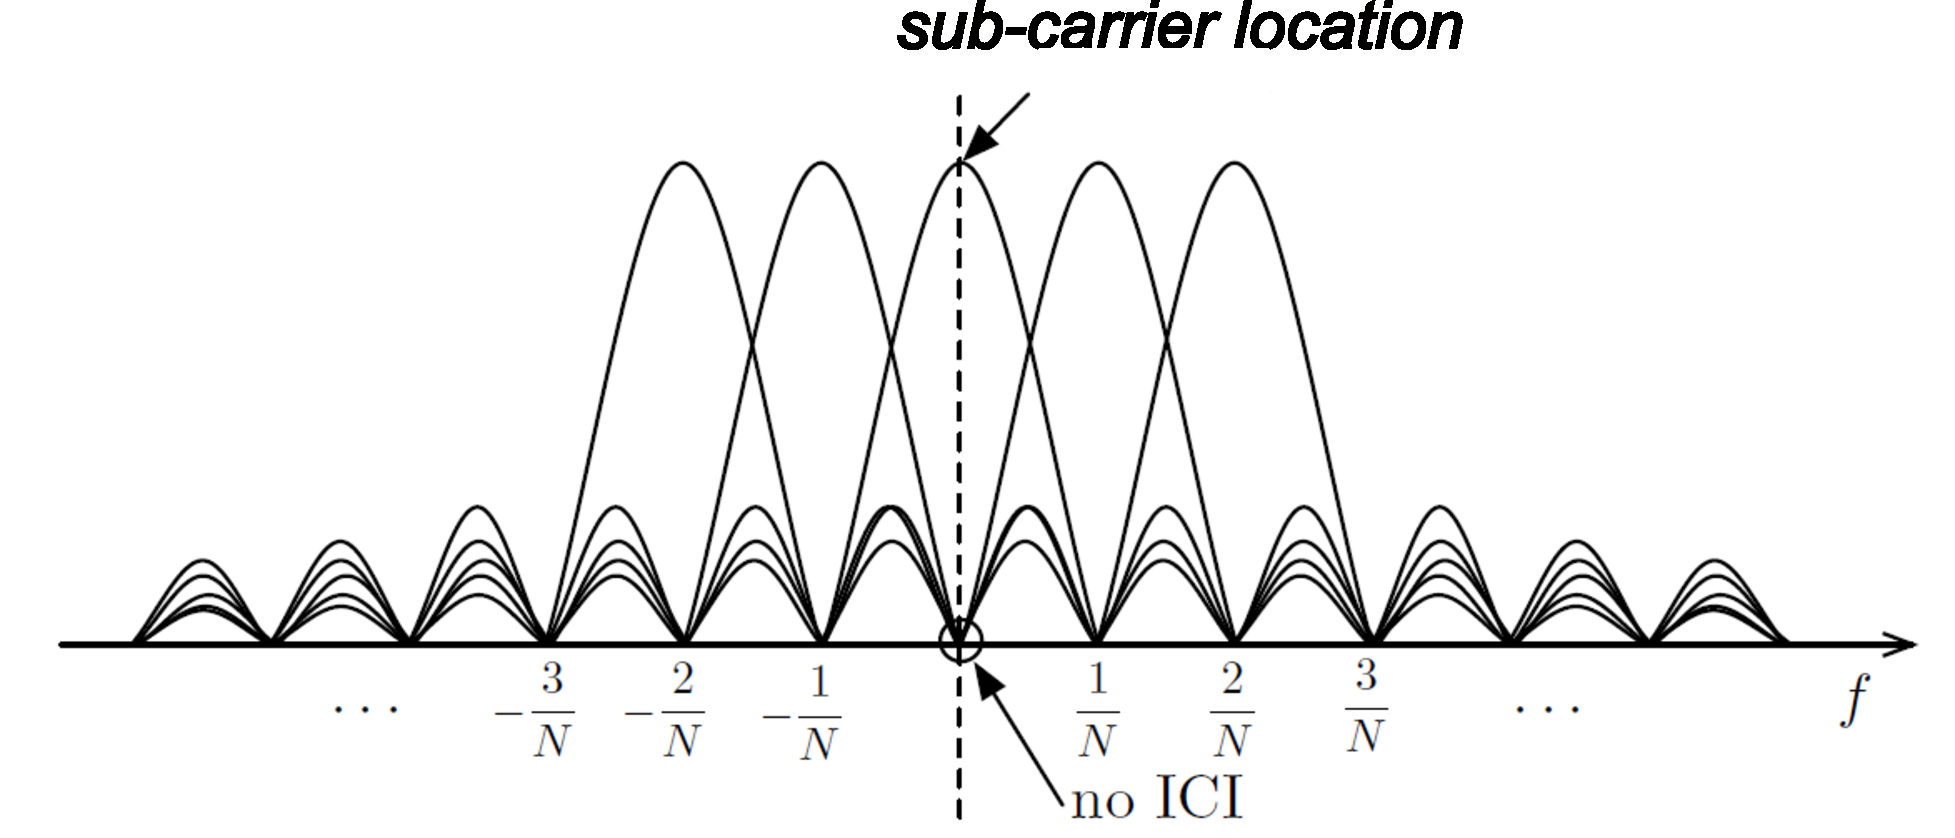
\includegraphics [width=0.8\columnwidth] {Figures/OFDM-subcarrier.pdf} }
	\caption{The spectrum of subcarriers in OFDM~\cite{farhang2008signal}.}
	\label{fig:OFDM-subcarrier}
\end{figure}

An OFDM symbol signal can be expressed at baseband as a sum of modulated complex exponentials:

\begin{eqnarray}
\label{equ:OFDMsignal}
s(t) = \sum_{k=0}^{N-1} X_k e^{i2\pi\Delta ft},
\end{eqnarray}
where $X_{k}$ represents a data modulated symbol such as a BPSK, QPSK, or QAM, and is a complex number modulated by the $k$th subcarrier of $N$ subcarriers and $\Delta f$ is the subcarrier spacing.
Sampling this OFDM symbol signal with sampling period of $T_S$ is expressed as:

\begin{eqnarray}
\label{equ:sampledOFDMsignal}
s(nT_S) = \sum_{k=0}^{N-1} X_k e^{i2\pi\Delta fnT_S},
\end{eqnarray}
A sample of the OFDM signal is equivalent to an inverse N-point discrete Fourier transform (IDFT), taking $X_{k}$ as a discrete point in the frequency domain.
Inversely, the sampled OFDM symbol signal can be demodulated using the discrete Fourier transform (DFT). OFDM modulation and demodulation are hence performed by computing the IDFT and DFT, respectively, expressed as:

\begin{eqnarray}
\label{equ:sampledOFDMsignal}
s[n] = \frac{1}{N}\sum_{k=0}^{N-1} X[k] e^{i2\pi\frac{k}{N}n},
\end{eqnarray}
\begin{eqnarray}
\label{equ:sampledOFDMsignal}
X[k] = \sum_{n=0}^{N-1} s[n] e^{-i2\pi\frac{k}{N}n},
\end{eqnarray}

In order to achieve efficient computation, The inverse Fast Fourier Transform (IFFT) and Fast Fourier Transform (FFT) are implemented in OFDM systems to modulate and demodulate the signal instead of the IDFT and DFT, respectively. These optimised algorithms generally rely on the number of points, and hence carriers, being a power of 2.

%---------------------------------------------------------------------------------
\subsection{The Cyclic Prefix}
%---------------------------------------------------------------------------------

When transmitting OFDM symbols over a delay-dispersive multi-path channel, the received signal is the linear convolution of the transmitted symbol with the channel impulse response (CIR)

\begin{eqnarray}
\label{equ:sampledOFDMsignal}
y[n] = h*s[n],
\end{eqnarray}

where $h$, assuming it has a length of $L$, denotes the equivalent impulse response of the channel. and $*$ is the convolution operation.
The received symbols $y[n]$ are the result of convolution between CIR $h$ and transmitted symbols $s[n]$ which has a length of $N$.
So, $y[n]$ has a length of $N+L-1$.
In addition, the received signal is obtained by concatenating the received OFDM symbols.
Because the received symbols, having a length of $N+L-1$, are overlapped with the adjacent received symbols, adding the overlap of adjacent received symbols leads to the introduction of inter-symbol interference (ISI) in the received signal, shown in Fig.~\ref{fig:CIR-noCP}.


\begin{figure}
	\centerline{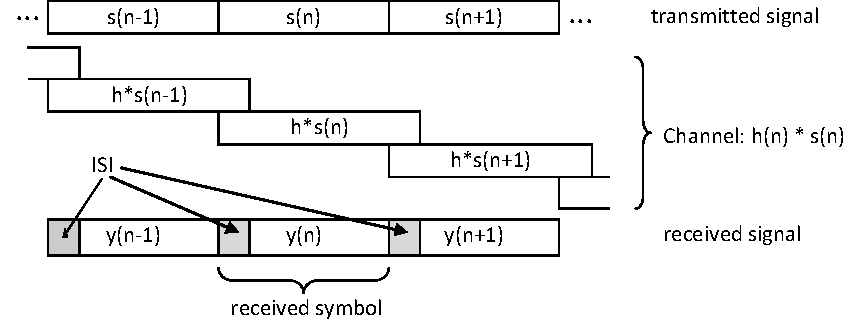
\includegraphics [width=0.8\columnwidth] {Figures/CIR_noCP.pdf} }
	\caption{OFDM transmission without cyclic prefix results ISI among adjacent symbol.}
	\label{fig:CIR-noCP}
\end{figure}

In order to avoid ISI, a guard interval (or cyclic prefix), having a length of $L_{CP}$, must be added before each OFDM symbol as demonstrated in Fig.~\ref{fig:CIR-CP}.
If the length of CIR, $L$, is smaller than that of the guard interval, $L_{CP}$, adding the overlap of adjacent received symbols will not interfere with the succeeding received OFDM symbol.
The ISI is hence missing in the received symbol.
The guard interval adopted in many OFDM standards can be commonly performed by a copy of the last $L_{CP}$ samples of the symbol as shown in Fig.~\ref{fig:CP}, that is called a cyclic prefix (CP).

\begin{figure}
	\centerline{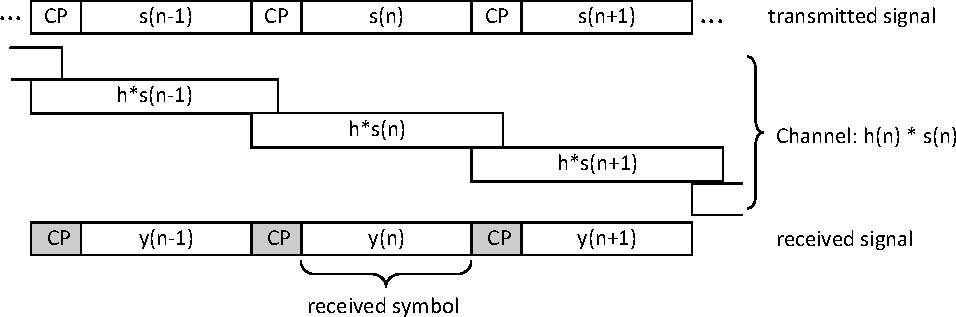
\includegraphics [width=0.8\columnwidth] {Figures/CIR_CP.pdf} }
	\caption{OFDM transmission with cyclic prefix avoids ISI among adjacent symbol.}
	\label{fig:CIR-CP}
\end{figure}

\begin{figure}
	\centerline{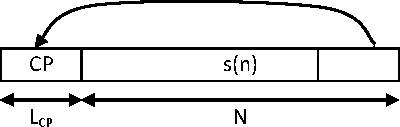
\includegraphics [width=0.4\columnwidth] {Figures/CP.pdf} }
	\caption{Inserting Cyclic Prefix in the OFDM symbol.}
	\label{fig:CP}
\end{figure}

In addition, the use of a CP also guarantees the orthogonality of subcarriers avoiding ICI. Performing the DFT operation and a single-tap equalizer per subcarrier allows recovery of the transmitted symbols~\cite{farhang2008signal}.

%---------------------------------------------------------------------------------
\subsection{OFDM Radio System}
%---------------------------------------------------------------------------------

An OFDM system model can be considered as shown in Fig.~\ref{fig:OFDM-model}.

\begin{figure}
	\centerline{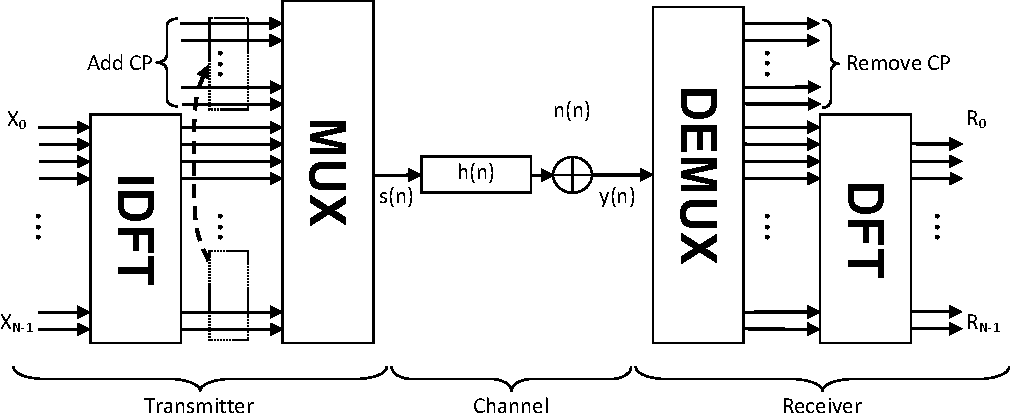
\includegraphics [width=0.8\columnwidth] {Figures/OFDM-model.pdf} }
	\caption{An OFDM system model.}
	\label{fig:OFDM-model}
\end{figure}

In the transmitter, the data modulated symbols $X[n]$ are grouped in blocks of $N$ sub-carrier symbols known as an OFDM symbol, expressed by a vector $X[n]=(X[1], X[2], ..., X[n])^T$.
Next, the OFDM symbol signal in the time domain is modulated by performing the IDFT on each OFDM symbol, and a cyclic prefix of length $L_{CP}$ is inserted at the begin of OFDM signal.
So, the complex signal of $m$, the OFDM-symbol in baseband discrete time, can be expressed as
\begin{eqnarray}
\label{equ:OFDMsymbol}
s_{m}[n] = \frac{1}{N} \sum_{k=0}^{N-1}X[k]e^{i2\pi k\frac{n-L_{CP}}{N}},
\end{eqnarray}

where $n$ is the discrete time index, $m$ denotes the index of the OFDM symbol.
The complete transmitted signal in the discrete time domain, $s[n]$, is given by the concatenation of all OFDM symbols, $s_{m}[n]$,

\begin{eqnarray}
\label{equ:OFDMsignal}
s[n] =  \sum_{m=0}^{\infty} s_{m}[n-m(N+L_{CP})],
\end{eqnarray}

When transmitting OFDM signals over a multi-path channel, the received signal is obtained through the linear convolution of the transmitted symbol with the CIR $h[i]$ and adding additive white Gaussian noise (AWGN) $n$.
Assuming that the synchronisation between the transmitter and receiver are perfectly achieved, the channel fading is slow enough to consider as a time invariant channel during one OFDM symbol interval, and the length of the cyclic prefix is longer than that of the CIR ($h[i] = 0$ for $i < 0 i > L_{CP}-1$),

\begin{eqnarray}
\label{equ:OFDMchannelsignal}
y[n] =  \sum_{i=0}^{L_{CP}-1} h[i]s[n-i] + n[n],
\end{eqnarray}

In the receiver, the incoming samples $y[n]$ are synchronously grouped into blocks of OFDM symbols and then the cyclic prefix in each OFDM symbol is removed.
The received symbols can be expressed in a vector $y_{m} = (y_{1}, y_{2}, . . . )$ , with $y_{m}[n]=y[m(Nc+Ncp)+Ncp +n]$.
The received data symbols associated with $m^{th}$ OFDM symbol $R_{m}[n]$ are retrieved by performing an $N$-point DFT:

\begin{eqnarray}
\label{equ:receiveOFDMsymbol}
R_{m}[n] =  \sum_{n=0}^{N-1} y_{m}[n]e^{-i2\pi \frac{nk}{N}},
\end{eqnarray}

\begin{figure}
	\centerline{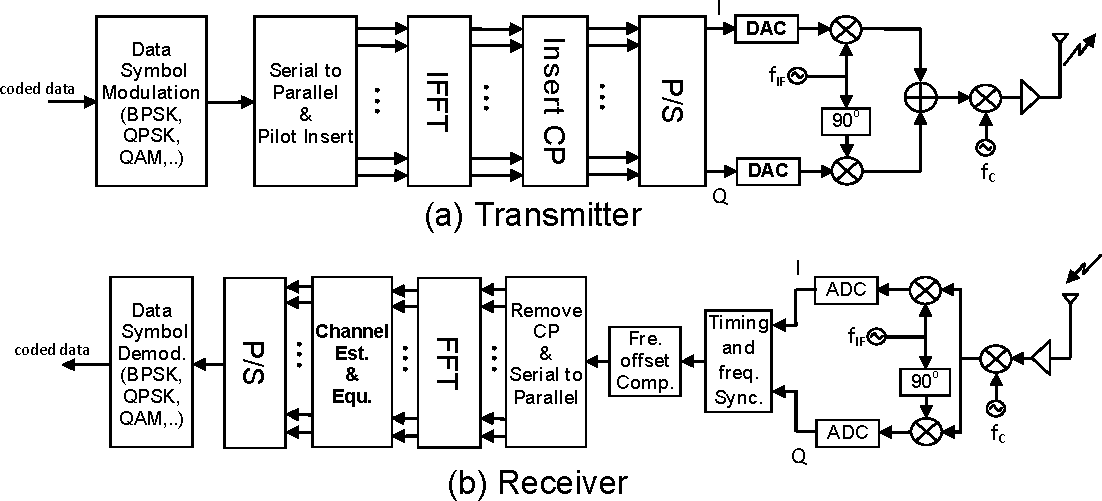
\includegraphics [width=0.8\columnwidth] {Figures/OFDM-block.pdf} }
	\caption{Block diagram of an OFDM radio system.}
	\label{fig:OFDM-block}
\end{figure}

Fig.~\ref{fig:OFDM-block} presents a common block diagram of an OFDM radio system.
OFDM is perform in the baseband, IFFT and FFT blocks are used to compute the IDFT and DFT for OFDM modulation and demodulation, respectively.
In the transceiver, the channel coded data from higher abstracted layers is modulated to data symbols (BPSK, QPSK, QAM, ...). The data symbols are then grouped together with the pilots to form $N$ FFT points in parallel.
After performing the IFFT, the CP is inserted, and then the OFDM samples are serialised and split in to in-phase (I) and quadrature (Q) channels corresponding to the real and imaginary parts of  the OFDM sample.
The digital to analogue converted signals of the I and Q channels are modulated by an intermediate frequency, $f_{IF}$, then the signal is up-converted to high frequency by an RF carrier, $f_{C}$.
Before transmitting, the signal should be amplified by an low noise amplifier (LNA).

In the receiver, after down-converting and I/Q demodulation, the signal is sampled. The samples are formed from I and Q channels corresponding to the real and imaginary parts of the OFDM sample.
The timing and frequency synchronisation blocks detect the frame start, recover timing of the frame and estimate the frequency offset.
The received samples are then compensated with estimated frequency offset in the discrete time domain.
After demodulating an OFDM symbol using the FFT, the channel is estimated and channel equalisation as well as phase error compensation are performed to improve performance.
The block of parallel samples in an OFDM symbol is serialised to data symbol sequences that are then demodulated, and coded data is sent to higher layers to decode.

%---------------------------------------------------------------------------------
\subsection{Evaluating OFDM}
%---------------------------------------------------------------------------------

The main advantages of OFDM are its spectrally efficient usage and robustness against multi path propagation.
This makes OFDM suitable for high performance wireless applications.
OFDM uses multiple sub-carriers which are overlapped with other subcarriers in the frequency domain, resulting in greater spectral efficiency than FDM.
Performing OFDM is equivalent to splitting a data stream into several parallel low-rate streams before transmission.
This makes the OFDM signal more robust against fading when transmitted through the channel.
Thanks to the cyclic prefix, the ISI and ICI caused by the multi-path channel can be eliminated.
The CP creates a guard period for an OFDM symbol, which should be longer than the CIR to ensure no ISI.
Repeating samples of the OFDM symbol in a guard period, the CP helps to maintain the orthogonality of subcarriers avoiding the ICI.
Thus, performing the DFT and a single-tap equalizer per subcarrier allows recovery of the transmitted symbols.

On the other hand, OFDM has some disadvantages.
Firstly, an OFDM signal is the sum of multiple modulated sub-carriers, and thus suffers a high peak-to-average power ratio (PAPR).
This results in demand on high power and wide range linearity in amplifiers increasing the cost of OFDM systems.
Secondly, the use of a guard period reduces bandwidth efficiency.
Last but not least, OFDM performance is sensitive to receiver synchronisation. Frequency offset causes inter-subcarrier interference and errors in timing synchronisation can lead to inter-symbol interference.
Much effort is needed to improve the accuracy of both frequency and time synchronizers for OFDM.



%-------------------------------------------------------------------------------------------------------------------------------------------------------------------------------------------------------------------------------------------------------------
\subsection{OFDM Synchronisation}
%-------------------------------------------------------------------------------------------------------------------------------------------------------------------------------------------------------------------------------------------------------------

OFDM performance is sensitive to receiver synchronisation.
Frequency offset causes inter-subcarrier interference, and errors in timing synchronisation can lead to inter-symbol interference, making synchronisation critical in OFDM systems.
There are two main errors implicit in synchronisation: sample clock timing offsets and carrier frequency offsets.
In order to obtain good synchronisation performance, timing offsets and frequency offsets must be studied in terms of their cause and effect on the degradation of OFDM received data symbols.
Additionally, there are issues of common phase error (CPE), generated from clock jitter and phase noise, that causes a random rotation of the entire signal constellation.
This must also be taken into account and compensated for in order to achieve good performance.

%---------------------------------------------------------------------------------
\subsubsection{Timing Offsets}
%---------------------------------------------------------------------------------

When sampling a signal at the receiver, the different times of sampling between samples in the receiver and transmitter are referred as timing error.
In a single carrier system, the symbol clock in the transmitter can be recovered at the receiver using a phase-lock loop (PLL)~\cite{farhang2008signal}.
This can correct a timing error in the receiver relatively easily.

In OFDM, however, timing errors comprise two categories: fractional and integer.
Fractional timing error, that is errors that are smaller than one sample period, are caused by different phases between the sampling clock of the analogue to digital converter (ADC) in the receiver and the phase of the transmitted signal, while integer timing error is that which is greater than one sample period, causing index shifting, or offset, in the sample sequence.

Timing error in the time domain is equivalent to a phase rotation in the frequency domain:

\begin{eqnarray}
\label{equ:timingoffset}
               s (t - \tau )   \Leftrightarrow  e^{-i2\pi f\tau} R(f),
\end{eqnarray}
where $\tau$ denotes timing error resulting in a phase shift of $e^{-i2\pi f\tau}$.
$s(t)$ is the received signal in the time domain, and $R(f)$ is the spectrum of $s(t)$ in the frequency domain.
The phase shift is proportional to both time errors and the frequency of carriers.
In the case of multi-carriers with increasing frequency, the phase shift is increased according to the carriers leading to the phase rotation of sub-carriers.
Carrier rotations caused by fractional timing error $\Delta t$ like those caused by fading can be estimated by a channel estimator and compensated for after performing the DFT:
\begin{eqnarray}
\label{equ:rotationcompensation}
               \widehat{R[n]} = R[n] e^{\frac{i2\pi n \Delta  t}{N}},
\end{eqnarray}
where $R[n]$, $\widehat{R[n]}$ denotes received data symbols before and after compensation, respectively. $\Delta t$ is estimated phase rotation, and N is the number of sub-carriers.

Moreover, the received samples in the receiver are synchronously grouped into blocks of OFDM symbols.
Integer timing errors lead to a symbol timing offset (STO) referring to the difference between the correct sample index and the actual sample index of received samples that causes a misaligned window for DFT demodulation in the receiver.
If the timing offset is late, the samples of the following symbol are used for the current symbol, resulting in ISI and hence degrading the performance of the OFDM system. The effect of ISI caused by later timing offsets on the OFDM received symbol is illustrated in Fig.~\ref{fig:Timingoffsetconstellation}(a) and Fig.~\ref{fig:Timingoffsetconstellation}(c).
If the timing offset is early, some samples in the CP of the current symbol are used to calculate the DFT, leading to sub-carrier rotation expressed in Equ.\ref{equ:timingoffset} in the frequency domain.
The effect of sub-carrier rotation caused by earlier timing offsets on the OFDM received symbol is illustrated in Fig.~\ref{fig:Timingoffsetconstellation}(b) and Fig.~\ref{fig:Timingoffsetconstellation}(d).

\begin{eqnarray}
\label{equ:rotationcompensation}
              s[n - t_{\mathit{off}}]  \Leftrightarrow R[n] e^{\frac{i2\pi n t_{\mathit{off}}}{N}},
\end{eqnarray}
where $s[n]$, $R[n]$ denotes received data symbols in the timing domain and the frequency domain, respectively. $t_{\mathit{off}}$ is a timing offset, and N is the number of sub-carriers.

\begin{figure}
	\centerline{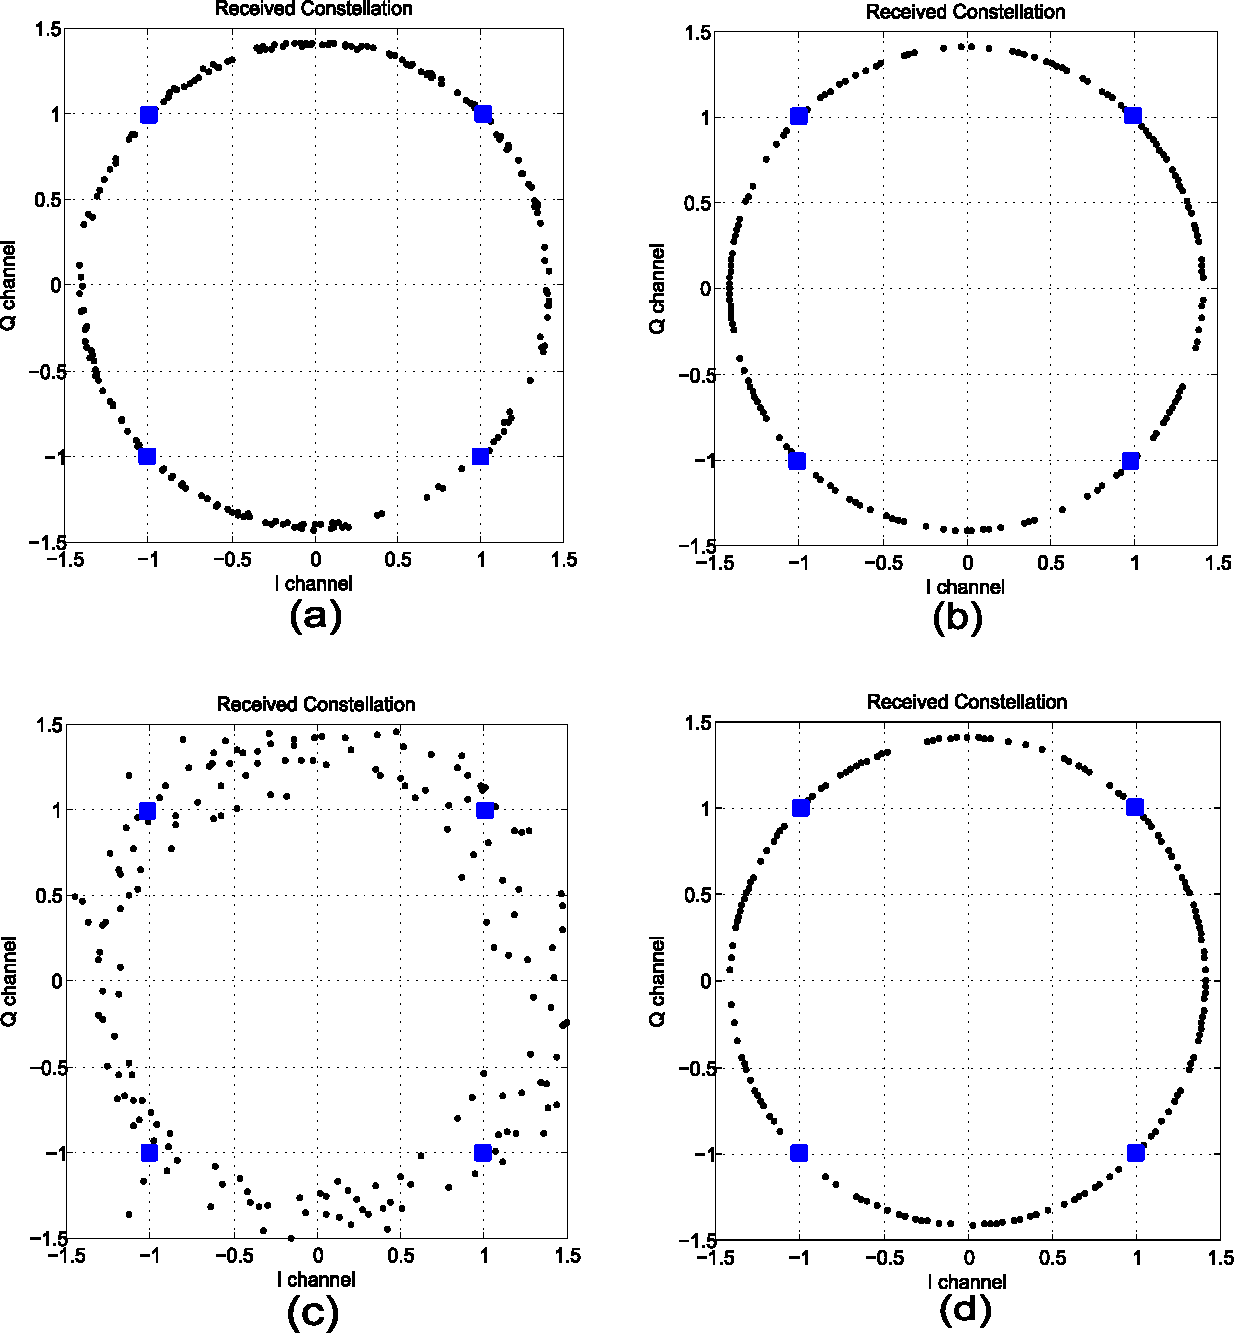
\includegraphics [width=0.8\columnwidth] {Figures/timeoff.pdf} }
	\caption{OFDM received symbol with timing offsets of -1, 1, -5 and 5 in a, b, c, d, respectively.}
	\label{fig:Timingoffsetconstellation}
\end{figure}

Fig.~\ref{fig:Timingoffsetconstellation} illustrates the effect of timing offset on a single 256 sub-carrier OFDM symbol utilizing QPSK sub-carriers (based on the IEEE~802.16 standard).
As can be seen, the earlier timing, for instance timing offsets of 1 and 5, shown respectively in Figs.~\ref{fig:Timingoffsetconstellation}(b) and~\ref{fig:Timingoffsetconstellation}(d), cause a carriers rotation similar to that of fractional timing errors, and fading that can be estimated by a channel estimator.
However, the later timing, for instance timing offsets of 1 and 5, as shown in Figs.~\ref{fig:Timingoffsetconstellation}(a) and~\ref{fig:Timingoffsetconstellation}(c), lead to ISI that prevents the OFDM constellation from being recovered.

Therefore, timing synchronisation is required to correct the timing offset, and avoid ISI.
Correlation is commonly performed to estimate timing offset~\cite{Dick2003,Fort2003,Wang2004}. One of the contributions in the thesis proposes a novel low-power correlation for OFDM synchronisation. The related work and proposed correlation are discussed in Chapter~\ref{chap:multiplierlesscorrelator}.
The accuracy of timing synchronisation also depends on the timing metrics and the algorithms applied on these metrics. A novel efficient and robust timing synchronisation based on the low-power correlation is proposed in this thesis. The related work~\cite{Schmidl1997,Kishore2006,Guffey2007,Huang2010,Recio2010} and proposed method for timing synchronisation will be discussed in Chapter~\ref{chap:Synchronisation}.
%---------------------------------------------------------------------------------
\subsubsection{Frequency Offset}
%---------------------------------------------------------------------------------

Carrier frequency offset (CFO) refers to a difference in frequency between the receiver clock with respect to the `correct' frequency of carriers in a transmitted OFDM symbol.
CFO is introduced due to an imperfect clock in the RF front-end, as well as by frequency variation caused by the Doppler effect when a signal is transmitted through a frequency selective channel.
This leads to the misalignment of sampling in sub-carriers in the frequency domain that causes a loss of orthogonality because at the point of frequency offset in the sub-carrier, the other sub-carriers are not null as expected (shown in Fig.~\ref{fig:OFDM-subcarrier-freoff}).
CFO is normalised by sub-carrier spacing and usually divided into an integer part (IFO), as a multiple of sub-carrier spacings, and a fractional part (FFO).
IFO causes a circular shift of the sub-carrier in the frequency domain while FFO results in ICI because of lost orthogonality between sub-carriers.

\begin{figure}
	\centerline{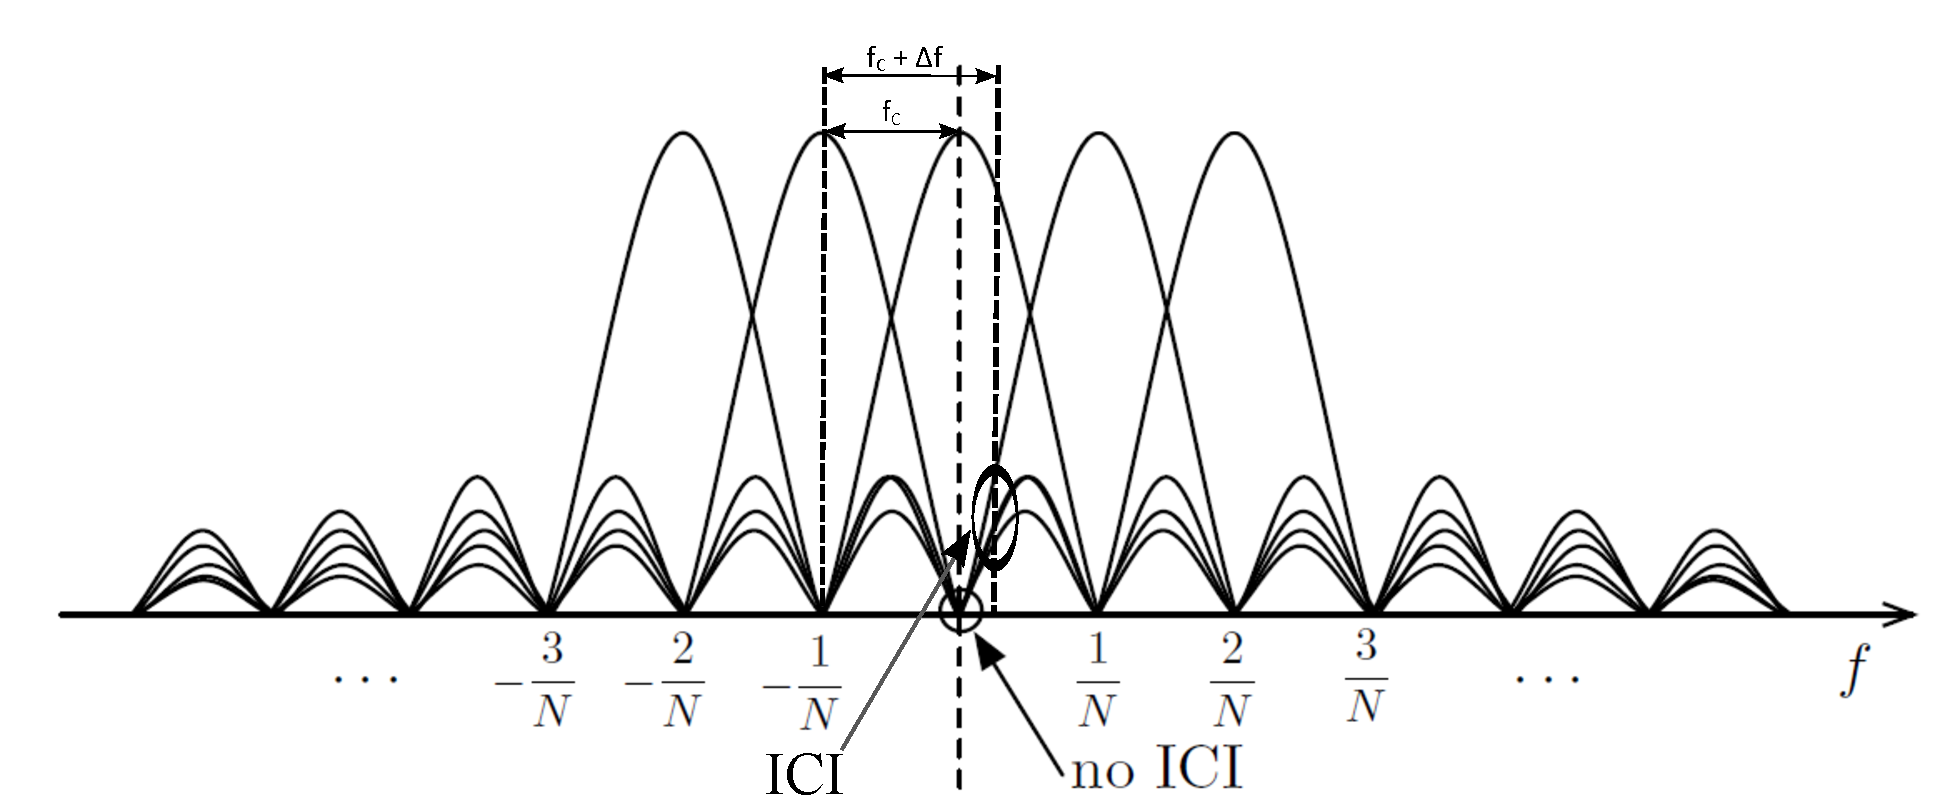
\includegraphics [width=0.8\columnwidth] {Figures/OFDM-subcarrier-freoff.pdf} }
	\caption{Inter carrier interference (ICI) caused by frequency offset $\Delta f$.}
	\label{fig:OFDM-subcarrier-freoff}
\end{figure}

With no frequency offset, the frequency bin of the DFT will be sampled at  the peak of each sub-carrier, $sinc(x)$ pulse, and other adjacent pulses are null at this point.
However, if frequency offset is introduced, the frequency bin of the DFT will sum the energy from other sub-carriers.
This means that the adjacent sub-carrier introduces an interference component resulting in ICI.

As can be seen, the adjacent sub-carrier introduces an interference component that is about half the amplitude of the sub-carrier of interest.
All other sub-carriers introduce an interference component of much lower amplitude.
This is known as a loss of orthogonality, and must be compensated for in order to properly demodulate the OFDM symbol.
The effect of CFO can be easily considered in the time domain by taking an inverse Fourier transform expressed as follows:

\begin{eqnarray}
\label{equ:}
             R(f - \Delta f) \Leftrightarrow  e^{i2\pi \Delta ft} s(t),
\end{eqnarray}

In the discrete time domain, the signal sample sequence can be expressed:
\begin{eqnarray}
\label{equ:}
            s[n]' = s[n] e^{\frac{− i2\pi \Delta fn}{N}},
\end{eqnarray}
where $s[n]'$ and $s[n]$ are the frequency offset samples and the original samples, respectively.
$\Delta f$ denotes the frequency offset, and $N$ is the number of sub-carriers.

The effect of frequency offset is shown in Fig.~\ref{fig:freoff_1sym}. Each plot illustrates the constellation of QPSK symbols demodulated from one 256 sub-carrier OFDM symbol based on the IEEE~802.16 standard.

\begin{figure}
	\centerline{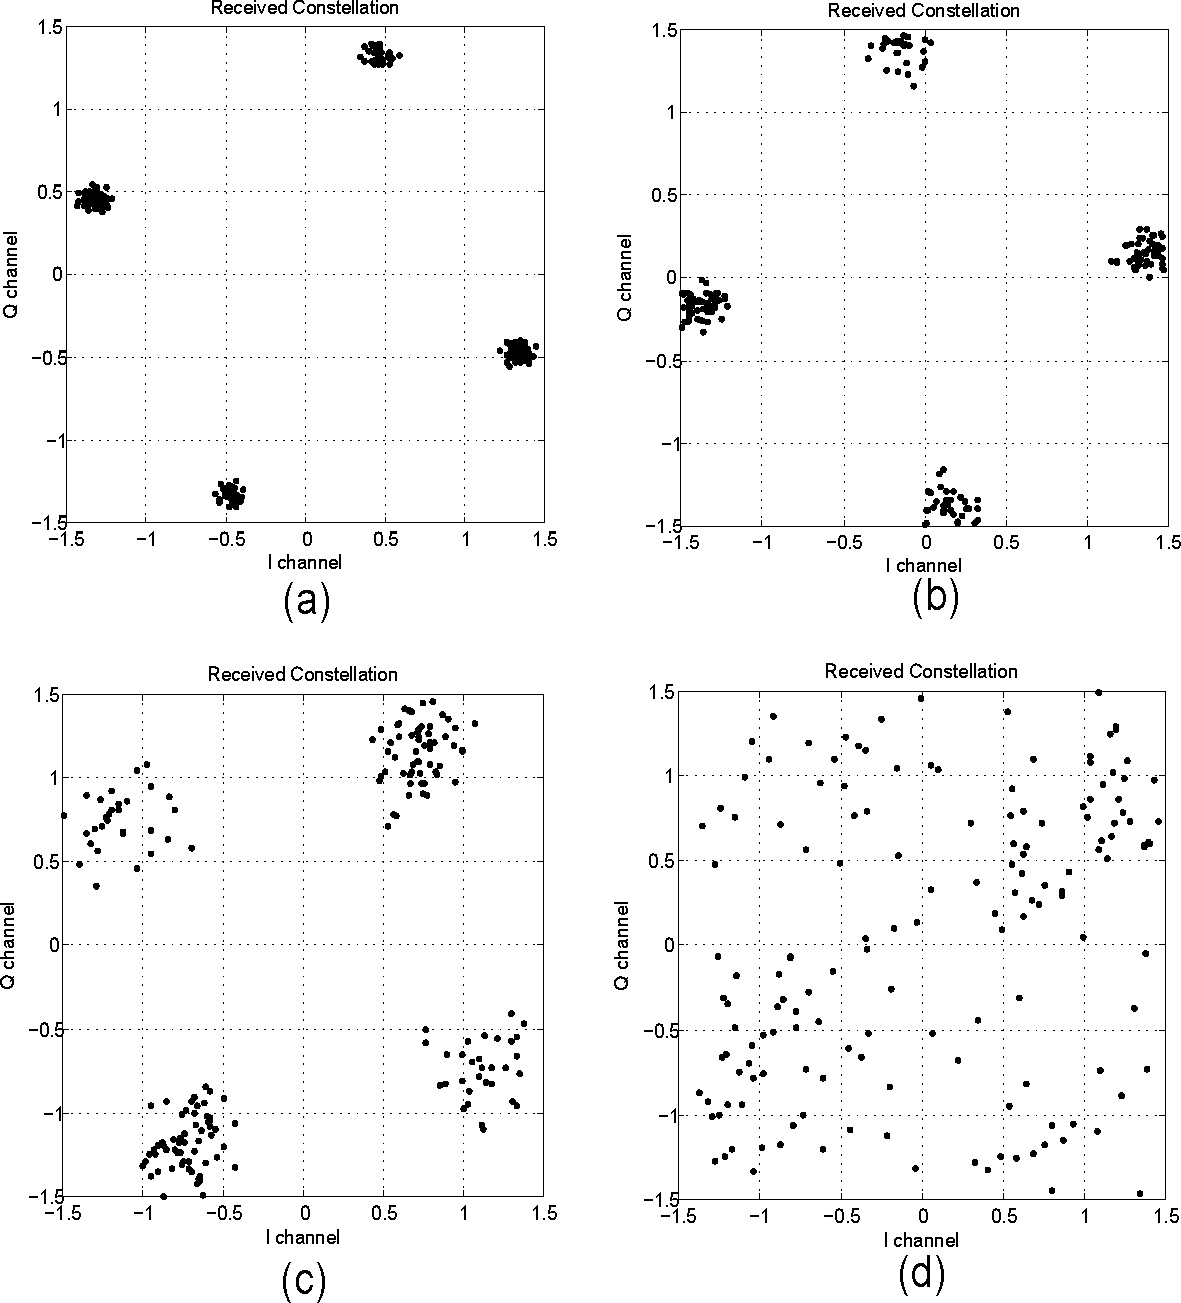
\includegraphics [width=0.8\columnwidth] {Figures/freoff_1sym.pdf} }
	\caption{The constellations of OFDM received symbol with frequency offets of 0.025, 0.5, 0.1 and 0.25 sub-carries spacing in a, b, c, d, respectively.}
	\label{fig:freoff_1sym}
\end{figure}

As can be seen, OFDM performance is sensitive to even small frequency offsets.
The effect of CFO causes dispersion, similar to AWGN, and also phase rotation in the QPSK constellation demodulated from the OFDM symbol.
If multiple data symbols are transmitted in a packet, the phase rotation of each OFDM symbol increases, and even small CFO will lead to a large drift of constellation points, shown in Fig.~\ref{fig:freoff_5sym}, degrading the performance of demodulation. CFO must be estimated and compensated for, in order to properly demodulate the OFDM symbol.

\begin{figure}
	\centerline{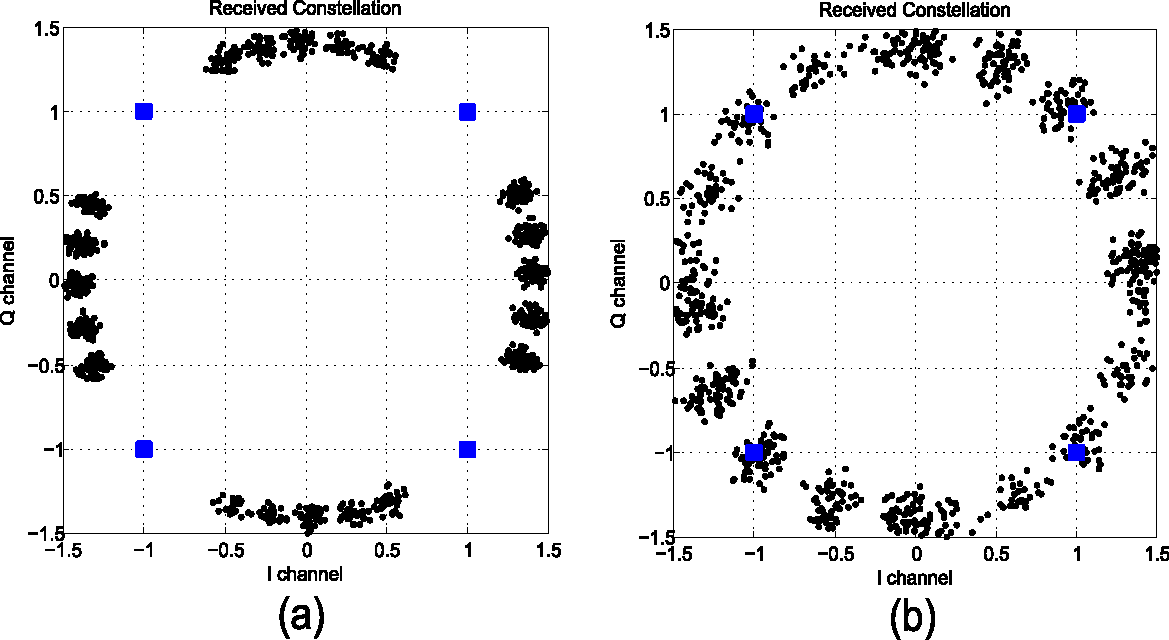
\includegraphics [width=0.8\columnwidth] {Figures/freoff_5sym.pdf} }
	\caption{The constellations of 5 consecutive OFDM received symbols with frequency offsets of 0.025 and 0.05 in a, b respectively.}
	\label{fig:freoff_5sym}
\end{figure}

Most published OFDM implementations limit their synchronisation to dealing with small CFO that can be corrected along with FFO.
Although IFO estimation methods have been explored in theory~\cite{Shim2006,Morelli2008,You2010,Lee2013,Morelli2014}, their implementation in hardware has not been published in the research literature primarily due to high computational complexity. In Chapter~\ref{chap:CFO}, we present a low cost, low power IFO estimation architecture for more robust OFDM synchronization.

%---------------------------------------------------------------------------------
\subsubsection{Phase Noise}
%---------------------------------------------------------------------------------

The intrinsic imperfection of the local clock at the RF front-end of a receiver or clock jitter of an ADC may introduce parasitic phase noise which can affect the performance of baseband data symbols, such as QPSK, QAM, ..., during demodulation.
Phase noise can be considered in two different parts: common phase error and inter-carrier interference~\cite{Armada1998}. The effect of phase noise can be expressed in the discrete time domain as:
\begin{eqnarray}
\label{equ:}
            s[n]' = s[n] e^{i\phi[n]},
\end{eqnarray}
where $s[n]’$ and $s[n]$ are the frequency offset samples and the original samples, respectively.
$\phi[n]$ denotes the phase noise.

If the phase noise is varying more slowly than the OFDM symbol interval, it can be considered a constant phase term added to each sample resulting in CPE~\cite{Armada1998}.
However, if the phase noise is varying much faster than the OFDM interval, different phase noise is added to each sample causing the loss of orthogonality, and thus, inter-carrier interference.
Fig.~\ref{fig:phasenoise} illustrates the effect of phase noise on baseband data symbol demodulation in an OFDM received symbol and 5 consecutive OFDM received symbols.
\begin{figure}
	\centerline{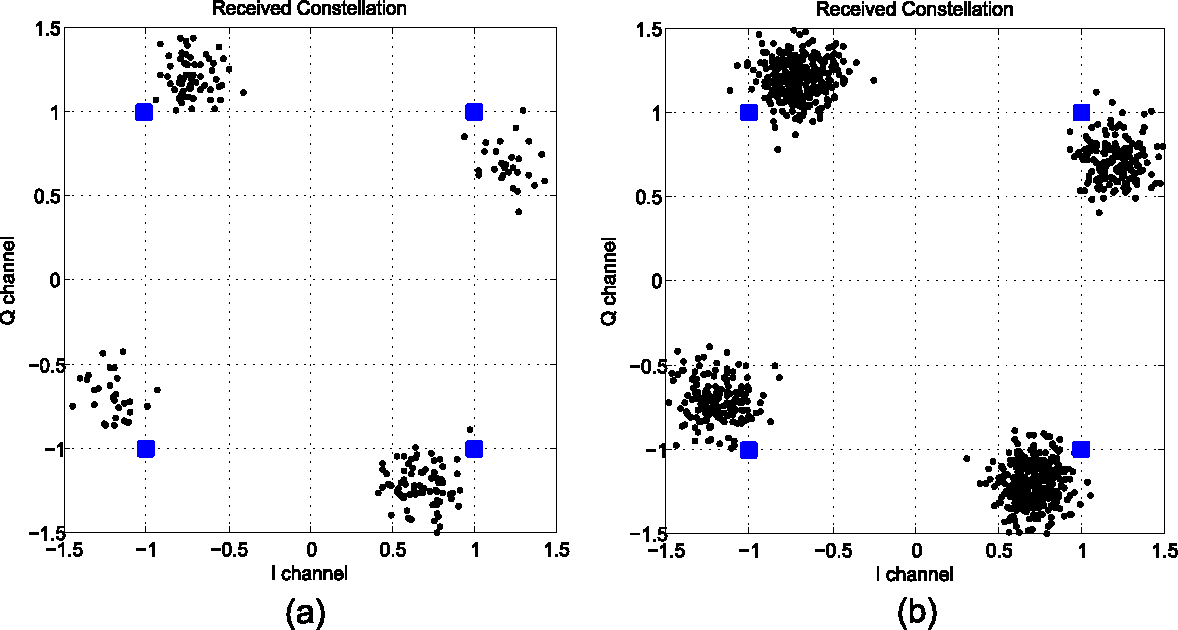
\includegraphics [width=0.8\columnwidth] {Figures/phasenoise.pdf} }
	\caption{The constellations of an OFDM received symbol and 5 consecutive OFDM received symbols with phase noise variance of 0.25 $rad^2$ in (a), (b) respectively.}
	\label{fig:phasenoise}
\end{figure}

As can be seen in Fig.~\ref{fig:phasenoise}, the degradation of OFDM demodulation includes two different phenomena affected by phase noise.
First, the constellations of the data symbol are rotated similarly to the effect of fractional timing error or residual frequency offset.
Second, the constellations of data symbols are dispersed like the effect of AWGN, causing a loss of orthogonality between sub-carriers.
However, the difference from the effect of frequency offset will be a constant constellation rotation for all OFDM symbol instead of a different constellation rotation for each symbol in the case of frequency offset.


%------------------------------------------------------------------------------------------------------------------------------------------------------------------------------------------------------------------------------------------------------------
\subsection{Shaping OFDM Spectral Leakage}
\label{Ch2:SpecLeak}
%------------------------------------------------------------------------------------------------------------------------------------------------------------------------------------------------------------------------------------------------------------

One drawback of OFDM is spectral leakage due to the summation of sinusoidal sub-carriers windowed by a rectangular function.
Some recent OFDM-based standards demand very strict requirements on spectral leakage to avoid inter-channel interference between adjacent transmission channels.
This raises a significant challenge in terms of how to shape the spectrum of the OFDM signal.

\subsubsection{Spectrum Emission Masks in Recent Standards}
In 2009, the FCC issued regulatory rules for reusing television white space (TVWS) spectrum.
IEEE~802.11af was developed under the 802.11 Working Group as a standard that enables a Wi-Fi service in TVWS spectral regions~\cite{802-11af2013}.
The scope of the standard is to define amendments to the high throughput 802.11's PHY and MAC layers to meet the requirements for channel access and coexistence in the TVWS regions.
One of the main challenges is the stringent spectral emission mask (SEM) requirements that are mandated by the FCC for these services.
Re-using existing 802.11 standards means hardware can be cheap, but the high throughput 802.11 scaled SEM is significantly inferior to the required spectral emissions shape for TVWS~\cite{Shellhammer2009}.
For instance, the 802.11 scaled SEM requires an attenuation of 20\,dB at the edge of the channel whereas the equivalent requirement for portable TV band devices (TVBD) is 55\,dB.

In 2010, the IEEE defined a standard for PHY and MAC layers~\cite{802-11p2010}, named IEEE~802.11p, for Dedicated Short-Range Communications (DSRC), the wireless channel for new vehicular safety applications through vehicle-to-vehicle (V2V) and Road to Vehicle (RTV) communications.
The PHY in 802.11p is largely inherited from the well-established IEEE~802.11a OFDM PHY, with several changes aimed at improving performance in vehicular environments.
The advantage of building on 802.11a is a potential significant reduction in the cost and development effort necessary to develop new 802.11p hardware and software.
It also plays an important role in allowing backwards compatibility from 802.11p to 802.11a~\cite{Vandenberghe2011,Fernandez2012}.
Essentially, three changes are made in IEEE~802.11p~\cite{Jiang2008}:
First, 802.11p defines a 10\,MHz channel width instead of the 20\,MHz used by 802.11a.
This extends the guard interval to address the effects of Doppler spread and inter-symbol interference in a VC channel.
Secondly, 802.11p defines several improvements in receiver adjacent channel rejection performance to reduce the effect of cross channel interference that is especially important in dense vehicle communication channels.
Finally, 802.11p defines four SEMs corresponding to class A to D operations that are specified and issued in FCC~CFR47 Sections 90.377 and 95.1509.
These are more stringent than for current 802.11 radios, in order to improve performance in urban vehicle scenarios.
In addition, 802.11p will operate in the 5.9\,GHz DSRC spectrum divided into seven 10\,MHz bands.
This channelization allows the MAC layer to perform multi-channel operations \cite{WAVE2010}.
The mechanism allows safety and other applications to occupy separate channels to reduce interference.
The four strict 802.11p SEMs are defined to reduce the effect of ICI between the channels. %, shown in Fig.~\ref{fig:4SEM},
Wu et al.~\cite{Wu2013} showed that transmitters on adjacent service channels still causes inter-channel interference (ICI) in the safety channel, even if they satisfy the class C requirement.
Shaping 802.11p spectral leakage is thus potentially important in helping to eliminate ICI.

\subsubsection{Dynamic Channel Requirements}
For static wireless devices operating in licensed spectral regions, the characteristics of communication systems that are licensed to occupy adjacent bands may be known.
Hence, spectral leakage masks for ICI avoidance in neighbouring systems can be statically specified.
However, in the case of shared and reused spectrum, the authors of SEMs should be defined in a more general and flexible way~\cite{Macaluso2014}.
In other words, CRs operating in dynamic spectrum access (DSA) environments must adapt their current transmission SEMs based upon their current operating region -- another argument for baseband digital filtering.
More sophisticated examples of SEMs are studied in \cite{Forde2010}, which deals with the broader concept of dynamic SEMs.

Time-varying SEMs may also need to consider that neighbouring systems are themselves able to change their SEMs, and hence through negotiation with each other change their masks for in- and out-of-band emission levels separately in accordance with their mutual temporal variations (for example, to adapt to communications traffic density or spatial deployment density).
In such future systems, an SEM defined by the regulator may simply be a starting point in a collaborative process in which neighbouring communication systems negotiate and renegotiate new SEMs as their status changes (e.g. to optimise computational power or increasing throughput).

Unfortunately, \cite{Forde2010} did not present a complete solution for dynamic filtering of spectral emissions, however they discussed deactivating sub-carriers or changing transmission power to satisfy the requirements of a dynamic SEM.
The former solution leads to a reduction in throughput due to reduced spectral band occupancy, whereas the latter impacts range.
A combined approach was presented in \cite{Kryszkiewicz2013} where some sub-carriers are reduced in power instead of being deactivated, in order to reduce spectral leakage to adjacent channels.

\subsubsection{Filtering in OFDM Implementations}
\label{sec:how_ofdm_works}

Modern OFDM implementations tend to favour subsuming as much processing as possible within the baseband digital components, in order to simplify the front-end RF hardware.
Although many alternative transmitter designs exist, direct up-conversion (DUC) architectures are commonly selected due to inherent implementation, cost and performance advantages~\cite{masse2006direct}.
Within the transmitter, orthogonal intermediate frequency (IF) signals are generated directly by digital baseband hardware, high-pass filtered and then quadrature up-converted to RF for transmission.
This contrasts with more traditional digital radio implementations in which the digital hardware generates baseband signals which are up-converted to IF in one or more analogue steps before conversion to RF.
Those systems would perform channel filtering predominantly with analogue filters, which require discrete precision components, and which tend to be inflexible in terms of carrier frequency and other characteristics.
For cognitive radio (CR) systems, where frequency agility is a requirement, and in SDR (software defined radio), both up-conversion to IF as well as channelisation filtering are performed in the digital domain~\cite{Chen2005,Dowle2006}.
Typically, this enables a relaxation of stringent IF and RF filtering requirements, which in turn allows a reduction in system cost, though requiring more complex signal processing.
A further advantage of baseband filtering is agility and flexibility.
In a CR context in particular, both channel and time agility are required, and this can be best achieved in the digital domain.

Within the baseband, OFDM symbols are constructed in the frequency domain and then transformed to a complex time domain representation through the IFFT.
A critically sampled construction process requires a sample rate of double the signal bandwidth.
This signal is up-converted to IF using an interpolation process, during which images of the original OFDM frequency response are created at integer multiples of the original sampling rate.
Image rejection filtering must then be performed on this signal prior to being output by the digital-to-analogue converters (DACs) and subsequent transmission, since the images lie out-of-band (OOB) and hence are a cause of ICI.

However any such filtering induces time-domain smearing of the transmitted signals~\cite{Faulkner2000} which adds to the similar effects caused by the channel impulse response (CIR) between transmitter and receiver, all of which potentially induce inter-symbol interference (ISI).

OFDM systems combat ISI by dividing information finely in the frequency domain across sub-channels to implement narrow (in frequency) but long (in time) transmitted symbols, and then providing a guard interval between successive symbol blocks.
The guard interval is determined by the duration of the expected channel and filter impulse responses that are traversed by each symbol on the path from transmitter baseband to receiver baseband.
The guard interval typically contains a cyclic prefix (CP) which is inserted to combat another cause of ISI: received frequency components ringing during the CIR due to the abrupt onset of modulation at the beginning of each symbol.
%
The nearly rectangular OFDM symbols in the time domain naturally have a frequency domain response consisting of overlapping Sinc shapes, complete with large side lobes that lie outside the main frequency channel.
These are another source of OOB interference which contributes to ICI.
As noted previously, both 802.11p and 802.11af (in common with most OFDM-based standards) specify an SEM which requires that ICI is controlled.

%\subsection{Spectral Leakage Compression}
%Conventionally, there are two methods that can be employed to compress the spectral leakage for OFDM-based system, namely pulse shaping and image spectrum compression. Pulse shaping, recommended in 802.11a, is effective at reducing side lobes.
%Considering an OFDM symbol to have IFFT length and CP length $N$ and $N_{CP}$, respectively, the length of the symbol including its CP is $N_{T} = N + N_{CP}$,
%a sample $x[m]$ of the OFDM symbol $(0\leq m \leq N_{T}-1)$ can be expressed in the time domain as,
%\begin{equation}
%\label{xm}
%x[m] = \frac{1}{N}\sum_{k=0}^{N-1} X[k] e^{i2\pi\frac{k}{N}(m-N_{CP})},
%\end{equation}
%where $X[k]$ denotes the frequency domain representation of the data sub-carriers.
%Since OFDM symbol samples are generally transmitted sequentially, this is equivalent to multiplying symbols with a rectangular window function, $p$.
%Then the transmitted OFDM samples can be expressed as;
%\begin{equation}
%\label{equ:xn2}
%x[n] = \frac{1}{N}\sum_{l=-\infty}^{\infty} \sum_{k=0}^{N-1} X[k] p[n-l N_{T}] e^{i2\pi\frac{k}{N}(n-N_{CP}-l N_{T})}
%\end{equation}
%In a conventional OFDM system, the window function, $p(m)$, is rectangular and simply described as;
%\begin{equation}
%\label{equ:pm}
% p[m] =\begin{cases}1, & m = 0,1, ..., N_{T} \\  0, & otherwise \end{cases}
%\end{equation}
%In pulse shaping OFDM, the window function, $p[m]$, uses a smooth rather than rectangular pulse resulting in inducing distortion in the subcarriers.
%One way to avoid this is to add extending parts, i.e. CP and a cyclic suffix (CS) before and after each conventional OFDM symbol respectively, and to multiply the extended symbol with a smoothing function.
%While the CP in conventional OFDM is used as a guard interval, here it is also used for pulse shaping. Pulse shaping extends the  $N_{T}$ length of the OFDM signal by a roll-off factor, $\beta$.
%The overhead of extending CS results in spectral loss; overlapping of the CP and CS of consecutive symbols shown in Fig.~\ref{fig:PS} is needed to form a transmitted symbol to reduce this loss, but causes ISI in the overlapped region. Pulse shaping using the overlapping method is effectively equivalent to shortening the OFDM guard interval.
%A larger $\beta$ obtains greater compression in spectral leakage but reduces the effective guard interval.
%When $\beta N_{T}$ is increased to equal the CP length, the effective guard interval is reduced to zero (no guard interval) to prevent channel-induced ISI.
%
%\begin{figure}[t]
%    \centerline{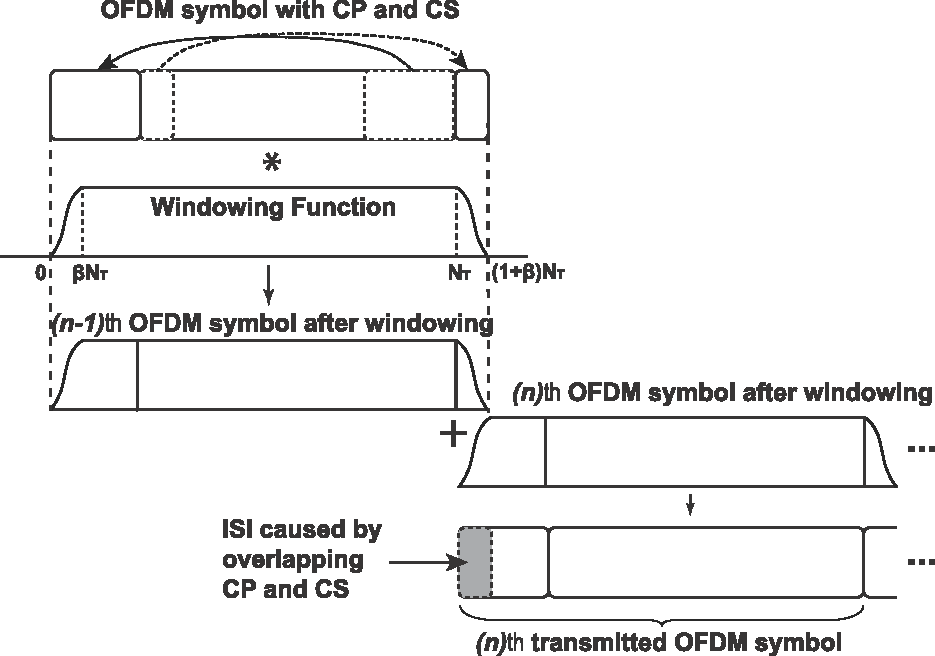
\includegraphics [width=0.9\columnwidth, height=7.5cm] {./Figures/w-ofdm.pdf} }
%	\vspace{-2mm}
%    \caption{Pulse Shaping operation performed on OFDM symbols.}
%    \label{fig:PS}
%\end{figure}
%
%Image spectrum compression is implemented as an FIR filter to cancel image spectra.
%The Interpolation can be used at baseband to increase sampling frequency, thereby extending baseband bandwidth.
%Image spectra are repeats of the original baseband spectrum, present because of interpolation or digital analogue converter (DAC) effects.
%On one hand, the narrow band gap between main and adjacent image spectra requires a long impulse response FIR filter.
%On the other hand, according to the performance of FIR expressed in (\ref{equ:FIR}), the impulse response of the FIR filter $h$ with length $L_{FIR}$ has a similar effect to the impulse response of the overall channel in terms of inducing ISI.
%\begin{equation}
%\label{equ:FIR}
%y[n] =  \sum_{i=0}^{L_{FIR}-1} h[i]x[n-i]
%\end{equation}
%
%The FIR filter reduces the effective guard interval of OFDM symbols~\cite{farhang2008signal}.
%Its design also needs to deal with the tradeoff between the length of filter to avoid ISI and the transition band and attenuation of the filter to meet the requirement of SEMs.

%-------------------------------------------------------------------------------------------------------------------------------------------------------------------------------------------------------------------------------------------------------------
\section{Field Programmable Gate Arrays }
%-------------------------------------------------------------------------------------------------------------------------------------------------------------------------------------------------------------------------------------------------------------
Field programmable gate arrays (FPGAs) are silicon devices with an architecture designed to be flexible enough to implement any type of circuit \cite{Kuon2008}.
They consist of programmable logic components coupled with configurable routing, and flexible I/O for interfacing with external components.
How these components and connections are set up is determined according to the contents of a configuration memory.
To implement a circuit, the designer typically describes it using a hardware description language like Verilog or VHDL.
Alternatively, tools exist that can map higher level languages like C or MATLAB Simulink directly~\cite{Springer2008}.
This description is then processed through synthesis and implementation tools, to determine a suitable mapping of the circuit to the components on the FPGA, and the connections between them.
This results in a bitstream that can be loaded into the configuration memory to set up the circuit described~\cite{Xilinx2013c}.
%---------------------------------------------------------------------------------
\subsection{FPGAs for Radio Platforms}
%---------------------------------------------------------------------------------
FPGAs have a long history of use in digital signal processing (DSP) applications.
They offer a way of exploiting the inherent parallelism in many DSP algorithms through custom architectures, resulting in significant speedup and efficiency compared to software based implementations.
On recent FPGAs, additional components like DSP blocks for high-performance signal processing improve performance further.
Generally, the designer will describe the architecture generally, and the implementation tools will decide when to use these components~\cite{Xilinx2013d}.

An exciting recent development is the emergence of new platforms that couple high-performance processors with a flexible FPGA fabric.
For example, the Xilinx Zynq family is a new generation of reconfigurable devices, which has a tightly coupled hardened 1 GHz dual-core ARM Cortex-A9 processor and reconfigurable fabric architecture along with several built-in peripherals~\cite{Xilinx2013}.
In such systems, the ARM can host a fully functioning software stack while the baseband can be implemented in the reconfigurable fabric. The connectivity between the two is very tight and offers high bandwidth and low latency. This represents an ideal platform for cognitive radio systems, offering both high computational performance and flexibility, while also facilitating a simple software programmable interface to higher layers of the radio.
A number of research groups are exploring ways to use these platforms in cognitive radios~\cite{Dobson2014}.

Partial reconfiguration (PR) is also an advanced technique available in recent FPGAs which further provides the flexibility \cite{Sedcole2006,McDonald2008}.
By modifying only a portion of the configuration memory, it is possible to modify only some system functionality while the remainder continues to operate without interruption.
This allows portions of a circuit to be changed at runtime, and is ideally suited to applications like cognitive radio~\cite{Delahaye2007,Delorme2008}.
It is clear that PR has significant benefits for dynamic systems like cognitive radios.
However, the design process remains suitable only for FPGA experts.
Recent efforts have begun to bridge this gap, allowing a modular approach to PR design, with automated partitioning and floorplanning of the FPGA~\cite{Vipin2012,Vipin2013}.
Combined with the improving efficiency of high-level synthesis, this will enable radio designers with minimal FPGA experience to leverage their power and flexibility in the design of cognitive radios.

Reduced power consumption is another benefit of PR that is important in radio systems.
FPGA based systems consume power in proportion to the size of the device, resource utilisation and operating frequency.
PR based designs save resources, and may even allow use of a smaller FPGA, hence saving power.


%---------------------------------------------------------------------------------
\subsection{Power Dissipation on FPGA}
%---------------------------------------------------------------------------------
The increasing computational requirements, and growing requirements for deployment in portable devices have prompted serious attention to reducing the power consumption of systems, including radios with a focus on the physical layer.
High power dissipation by a system introduces high operating temperatures and follow-on effects that increase the cost of packaging as well as requiring larger batteries in the case of portable devices, or other power supply solutions.
Power dissipation has thus come to be considered as one of the most important design metrics, along with area and performance.
Reducing power consumption has been investigated at all levels of the digital design flow: from the system design stage to the layout stage.
At every stage, the designer can act to optimise the power consumption of the design.

However, small changes at the lower levels may require more work and time to update the higher level optimisations, thus increasing the complexity of the optimization process.
Moreover, at the system design level stage, the designer has more options to reduce power dissipation by a greater degree.
At the lower level, the architecture of the system is designed in terms of data flow between registers, leaving few options to optimize the system.
Thus, most power saving opportunities may exist at higher level of the design abstraction~\cite{Raghunathan1998}.

FPGAs, with their highly parallel architecture, are suitable for the increasing computational requirement of signal processing in wireless communication systems.
In order to optimise the power dissipation of systems on FPGAs, the power consumption of FPGAs needs to be clearly understood, and accurate, flexible power estimation tools are needed in order to provide power profiles of the system to help the designer makes the best decisions.
In addition, low power design techniques must be investigated to optimise power consumption when a system design is implemented.
%
%Fast time-to-market, flexible programmability, and improving performance continue to render FPGAs an attractive platform for digital circuit implementation.
%FPGAs have been gaining ground as an alternative implementation technology in a wide range of application domains, due primarily to the increased cost and diminished economies of scale when building custom ASICs.
%However, power remains a key metric in which FPGAs lag behind custom ICs, although this gap is narrowing.

Total FPGA power is calculated as follows:
\begin{center}
\begin{equation}
\label{Equ:Ptotal}
 P_{\mathit{total}} = P_{\mathit{device static}} + P_{\mathit{design static}} + P_{\mathit{dynamic}},
\end{equation}
\end{center}
where $P_{\mathit{total}}$ represents the total power consumption, $P_{\mathit{device static}}$ refers to the leakage power which is proportional to the size of the device and resource utilisation when the device is powered, $P_{\mathit{design static}}$ is the additional power dissipation when the design is configured on the device and has no switching activity. Leakage current is the only source of this static power dissipation.
$P_{\mathit{dynamic}}$ represents the additional average power consumption from user logic utilization and switching activity caused by signal transitions in the design. Increasing operating frequency leads to a rise in switching activity and thus results in increased dynamic power consumption. The most significant source of dynamic power dissipation is the charging and discharging of parasitic capacitance as a result of signal transitions.

Efficient power-aware designs for FPGA-based systems require estimation tools that gauge power consumption at an early stage in the design flow.
These tools allow design tradeoffs to be considered at a high level of abstraction, thus reducing design effort and cost.
Significant research on FPGA power consumption has appeared in the literature~\cite{Shang2002,Anderson2004a,Anderson2004,Todorovich2005,Reimer2006}.
These papers have shown that power consumption of FPGA devices is predominantly confined to the programmable interconnect.
In the Xilinx Virtex-II family, for instance, it was reported that between 50-70\% of total power is dissipated in the interconnection network~\cite{Shang2002}.
The majority of power dissipation in FPGAs is dynamic power dissipation~\cite{Shang2002} as characterized by:

\begin{center}
\begin{equation}
\label{Pdynamic}
 P_{\mathit{dynamic}} =\frac{1}{2} \sum\limits_{i \in \mathit{all nets}} C_{i} \cdot f_{i} \cdot V^2,
\end{equation}
\end{center}
where $P_{\mathit{dynamic}}$ represents average power consumption, $C_{i}$ is the capacitance of a net, $f_{i}$ is the average transition rate (switching activity) of a corresponding net, and $V$ is the voltage supply.
Thus, estimating dynamic power (\ref{Pdynamic}) requires two parameters for each net: switching activity and capacitance.
The net's capacitance is the parasitic effect on interconnection wires. It depends on the used interconnect resources.
The switching activity represents the signal transitions on the net, depending on how circuit delays are accounted for.
Zero delay activity can be calculated assuming logic and routing delays are zero. Logic delay activity can be calculated considering only logic delays.
Routed delay activity can be calculated using complete logic and routing delays.
When delays are accounted for, the presence of glitches, which are spurious logic transitions due to unequal path delays to the net’s driving gate, leads to an increase in switching activity.
The additional activity due to glitching actually causes a significant increase in dynamic power~\cite{Anderson2004a}.
The path delays in FPGAs are also significantly dominated by interconnects, which have a different delay, compared to primitive logic delays. Therefore, the result of glitching on total power consumption may be more severe in FPGAs versus ASICs.

It is generally accepted that the dominant source of optimising power dissipation on FPGA is optimising dynamic power dissipation.
Dynamic power dissipation is proportional to switching activity and the equivalent capacitance of the circuit.
There are many techniques and strategies to reduce the power dissipation in FPGA presented in the literature~\cite{Danckaert1999,Kovacs2000,Czapski2007,Liu2009,Ahuja2010}.
However, only the strategies which appear to be suitable for wireless systems are discussed here.
These strategies will be discussed in detail for specific implementations in the following chapters, but the general approach is discussed here.

Firstly, in signal processing dominated systems, storing and transferring data between functional modules consumes a large proportion of total energy~\cite{Liu2009}.
The power consumption thus heavily depends on the way a system is partitioned and modularized and hence the use of data buffers to synchronously transfer data between functional modules.
In order to optimise power dissipation at a system level, such systems are often realized to support stream processing in which buffering data between functional modules requires much less memory.
The energy for storing and transferring data is thus reduced significantly.

Secondly, latching registers with enable signals should be used at the inputs of functional modules.
These can reduce switching activity inside functional modules when they are waiting for synchronization in a streaming process.
Power estimation tools should be used to evaluate the power dissipation of the system at each stage of the flow.
This provides information to assist in making decisions for reducing power dissipation.

%---------------------------------------------------------------------------------
\subsection{Power Estimation}
%---------------------------------------------------------------------------------

Several studies investigating power estimation techniques at different levels from the circuit level up to the system level have appeared in the literature.
At the circuit level, a circuit simulator such as SPICE~\cite{Deng1994} provides one of the most accurate power estimation methods, but the computational overhead involved in this is not really suitable for highly integrated and dense FPGA based systems and complex designs.

%A large amount of research has focused on logic-level power estimation \cite{Anderson2004a,Anderson2004,Todorovich2005}.
%Logic-level techniques can be classified into three categorises:  simulation-based techniques,  probability propagation techniques, and statistical techniques.
%
%Simulation-based techniques rely on simulating the logic response with specific input signals to compute the power consumption.
%The PowerPlay power analyzer integrated in Altera Quartus II \cite{ALTERA2010} and the XPower Analyzer integrated in Xilinx ISE Design \cite{XilinxXPOWERA2011} are both able to support computing of the switching activities of signals and dynamic power consumption from a simulation file;
%Secondly, probability-based propagation techniques calculate the value and transition probabilities of all logic signals in the circuit according to the given value and transition probabilities of the primary inputs from which the power consumption is estimated based on the computed probabilities.
%Statistical techniques such as Monte-Carlo simulation will monitor values of power consumption according to stimulating generated input patterns until it converges to within user-defined error and confidence levels. Todorovich et al. \cite{Todorovich2005} presented the development of a new FPGA-oriented power estimation tool based on this statistical approach.

%With increasing system complexity, several studies have recently paid attention to power estimation and optimization at higher level and earlier stages of the design such as the register-transfer and behavioural levels. The large run-times required by lower level power analysis tools, and the need to synthesize and validate a gate- or transistor-level netlist make previous techniques highly inefficient for exploring high-level design tradeoffs, and infeasible for use in automatic high-level and system-level synthesis and optimization tools.

Several studies have shown that the efficiency of power optimization is significantly better at the higher levels~\cite{Landman1996,Gupta2000,Raghunathan2003,Reimer2006}.
High-level power estimation is needed to conveniently validate power budgets for the different parts of the design and identify the most power hungry parts in the design and to quickly evaluate the effects of optimizations on the overall system power budget.
Furthermore, the long run time and and the complexity of synthesizing and validating a gate-level netlist makes lower level estimation approaches highly inefficient for exploring high-level design abstraction tradeoffs.

%%---------------------------------------------------------------------------------
%\subsubsection{High Level Power Estimation}
%%---------------------------------------------------------------------------------
%
%Power estimation performed at higher levels of design abstraction is more efficient due to the reduction in complexity of netlists in the design, and due to the availability of behavioural information which is more difficult to obtain at the lower levels.
%However it also introduces an accuracy penalty due to reducing the complexity of analysis.
%The absolute accuracy of high level power estimation is typically lower than the accuracy of estimation at the lower levels of the design hierarchy.
%
%Recently, more research has focused on the RTL/architecture level power estimation to obtain the power profile for optimizing at high level designs as well as for software programs. Raghunathan et al. \cite{Raghunathan2003} classified high level power estimation into three broad approaches, namely analytical models, control logic analysis techniques, and characterisation-based macro-modeling.
%At an architectural design level, different parts such as arithmetic macro blocks, control logic, memory, clock network, and I/O are analysed using different estimation approaches.
%
%Analytical power modelling techniques are based on correlating power consumption to measures of design complexity. These techniques may be used to estimate in the early stages of a design when complexity is known after synthesizing or mapping the design.
%For example, the design power estimation tool, XPower Estimator \cite{XPowerEstimator2011},  computes the dynamic power consumption of a logic block based on its used resource count, load capacitance per logic element, the clock frequency, and the average switching activity factor.
%The designer has to provide estimates for some of these parameters such as clock frequency and the average switching activity factor.
%The result depends significantly on the designer's judgment.
%Generally, such techniques are not highly accurate, however, they may be suitable for specific modules of a design such as memories for which the complexity parameters are easy to estimate and also can be used to estimate power in the early stages.
%
%Control logic analysis techniques consider the control logic parts of a design. The activity-based control model \cite{Landman1996} is an example of this approach.
%The switching activities of a control unit show significant spatial and temporal correlations to the remaining parts of a design.
%So computing the power consumed in the control logic and taking into account its impact on the design can estimate the power consumption of the design.
%Furthermore, since the control logic is typically smaller in size than the datapath, it can have low overheads and be fast to synthesis, followed by estimating its power consumption at a lower level.
%In addition, the glitching activity of the control signals have a significant impact on the power consumption in the rest of the design.
%
%Characterization-based macro-modeling is an approach mostly used in high level power estimation that uses a macro-model abstraction to obtain and characterize the power consumption of macro-blocks using the measure of lower level methods.
%A gate-level or logic-level power estimation tool is used to observe the power consumption of the macro-block for various input samples, called training sequences.
%Based on this observation, a macro-model is built, in which the macro-block's power dissipation is considered as a function of various selected parameters such as the statistics of the inputs and outputs.
%This approach is best suited for bottom-up design methodologies where models of macro-blocks instantiated from a component library can be used to estimated the power consumption of design.
%
%%---------------------------------------------------------------------------------
%\subsubsection{Xilinx Power Tool}
%%---------------------------------------------------------------------------------

The contemporary Xilinx FPGA design suite supports two power estimation tools: XPower Estimator (XPE) and  XPower Analyzer (XPA).
These tools provide the power profile of a system in the early stages when the RTL description is being implemented that helps the designer improve power characteristics when implementing the system.
XPE is a Microsoft Excel spreadsheet that is used to estimate power distribution typically used in the pre-design and pre-implementation phases of the design flow~\cite{XPowerEstimator2011} .
XPE supports selecting the relevant power supply and thermal management components based on the system's architecture evaluation and device selection.
XPE reads the resource usage of the implemented system, toggle rates, I/O loading, and many other factors from a designer's input and combines these with the appropriate device models to estimate power distribution.
The appropriate device models are obtained from measurements, simulation, and/or extrapolation.
There are two primary components that contribute to the accuracy of XPE.
One is the designer's input estimates such as toggle rates, I/O loading.
The other is device data models integrated into the spreadsheet that are selected based on the device selection.
Realistic input must be provided to obtain an accurate estimation.

As an early exploration tool, XPE's accuracy is heavily influenced by the numbers input by the designer.
After synthesis and implementation, XPA provides a more accurate estimation and power analysis.

XPA analyses the design on real design data from the system such as the (native circuit description (NCD) file output once the design has been fully implemented.
XPA employs a vectorless estimation algorithm in which the switching activity of nodes is assigned to appropriate values even if they are not defined in the input file.
However, simulation activity files such as a Value core dump (VCD) file from a functional simulation in timing mode are required for accurate power analysis.
These offer low-level switching activity for all signals in the design, factoring in timing delays.

The power profile of the system, including resource usage and the capacitance of nodes and nets is extracted from the NCD file, while switching activities are computed with high accuracy based on timing simulation from the VCD files. Much more realistic power information is obtained at this stage, thus, XPA can achieve more accurate results in terms power estimation.
XPA generates a text-based power report that shows the power distribution on the system that can used for optimisation.

Finally it is possible to measure power of a design loaded and functioning in an FPGA using lab equipment to monitor the currents on the various voltage rails. This can give a better view of overall board-level power.

%---------------------------------------------------------------------------------
%\subsection{Low power design strategies}
%---------------------------------------------------------------------------------


%------------------------------------------------------------------------------------------------------------------------------------------------------------------------------------------------------------------------------------------------------------
\section{Summary}
%------------------------------------------------------------------------------------------------------------------------------------------------------------------------------------------------------------------------------------------------------------

Reducing power dissipation has become a crucial issue in wireless communication systems, especially for portable devices.
In this chapter, the power consumption of FPGA systems is discussed.
The power estimation and analysis tools of Xilinx are also studied and employed in this research to evaluate the power dissipation of the researched system for power consumption optimisation.
Some low-power design strategies are suggested.
This chapter also provides the background of OFDM in terms of its mathematical representation and functionality, and then the advantages and limitations of OFDM are also discussed.
The concept of a MSRC based on OFDM techniques is presented. The challenges of implementing the MSCR system are introduced regarding the architecture and its performance.
The synchronisation effects on the OFDM performance are also considered.
Last but not least, the challenge in terms of OFDM spectral leakage are discussed in case of the strict requirements imposed by recent wireless standards.
